\documentclass[12pt,letterpaper]{article}
    \usepackage[utf8]{inputenc}
    \usepackage{ifpdf}
    \usepackage{mla}
    \usepackage[pass]{geometry}
    \usepackage{todonotes}
    \usepackage{graphicx}
    \usepackage[hidelinks]{hyperref}
    \usepackage{float}
    \urlstyle{same}

\begin{document}
\begin{mla}{Bernardo}{Meurer}{Professor Eckford-Prossor}{English 111 H}{April 02, 2018}{Essay 3 --- 321's}
    \subsection*{3 --- Quotations}
    \begin{itemize}
        \item ``I'm Lost'' ---
It is is interesting to see how the movie ends up showing that home is not real; home is abstract, always. Saroo, in his search for being ``found'', goes back to his home in Ganesh Talai, and finds his mother; but he is not himself ``found'', he remains lost.

Home is for him always an imaginary entity that surrounds his brother, Gudu, his Mother, his sister, his village, and his lifestyle as a poor child in Ganesh Talai. Home is the product of this multitude of factors, as experienced, and most importantly remembered, by Saroo. Yet when he returns to Ganesh Talai everything has changed; his brother is dead, his mother is old, his sister has grown, his house is now a goat stable, the language is unintelligible. He may have found his mother, and his hometown,  but he has not found home, for that no longer exists. It is in this sense that Saroo remains lost, and unchangeably so, for he is unable to reconnect his self present with his self past, for the conjuncture that defined the latter is gone.
        \item ``As she left, she looked at me over her shoulder, my heart trampolined, and she followed others into the street.'' (Mitchell 42)
    --- This reminds me of the Baudelaire poem ``À une passante,'' Translated to English as ``To a Passer-By,'' that explores throughly the idea of the sudden and spontaneous love that happens in the city, relating in many ways to Baudelaire's image of the *flâneur* as well. I've felt this myself, and related to Baudelaire, of being walking around the city, commuting perhaps or headed somewhere, nowhere, and seeing the most absolutely beautiful woman, the breathlessness, the impatience, to think we could love each other and perhaps be true soulmates, only to have her jump off the train in the next station, into the complete void of oblivion.
    This can also be observed in the works of Portuguese poet Cesário Verde, whose statue I passed by every morning for the year I lived in Lisbon, but whose work until now I had never bothered reading. In his poem ``Num Bairro Moderno'', which translates as ``In a Modern Neighborhood,'' Cesário works through the minutia of a day in modern life, and of the `known unknowns'' that are others.
    In another of his poems, ``Deslumbramentos'' or `Dazzles'' (Note that I do not believe that ``Dazzle'' is a fair translation of the Portuguese original, but after much thought I have failed to come up with any better alternative, and therefore will use ``Dazzles'') he explores the dangers of contemplating an unattainable love.
    I'm not sure where to go with this, but I feel like with some more thought I might be able to connect this to how we understand who we are, or at least with the ``cognitive dissonance'' of the city. Also, this point makes me think of Chopin's Preludes, not entirely sure how to relate it rigorously yet.
\item When Saroo returns to his hometown --- This is an interesting scene because it depicts the immutability of home proper, as opposed to the mutability of home real. Similar to the home / house distinction, his home is permanent, even when it's physical anchor, his house, is gone. It's interesting to see how finding his long lost family is what, it seems, brings him closer to home; not the location itself.
    \end{itemize}
    \newpage
    \subsection*{2 --- Questions}
    \begin{itemize}
        \item What is home?
            \begin{figure}[H]
            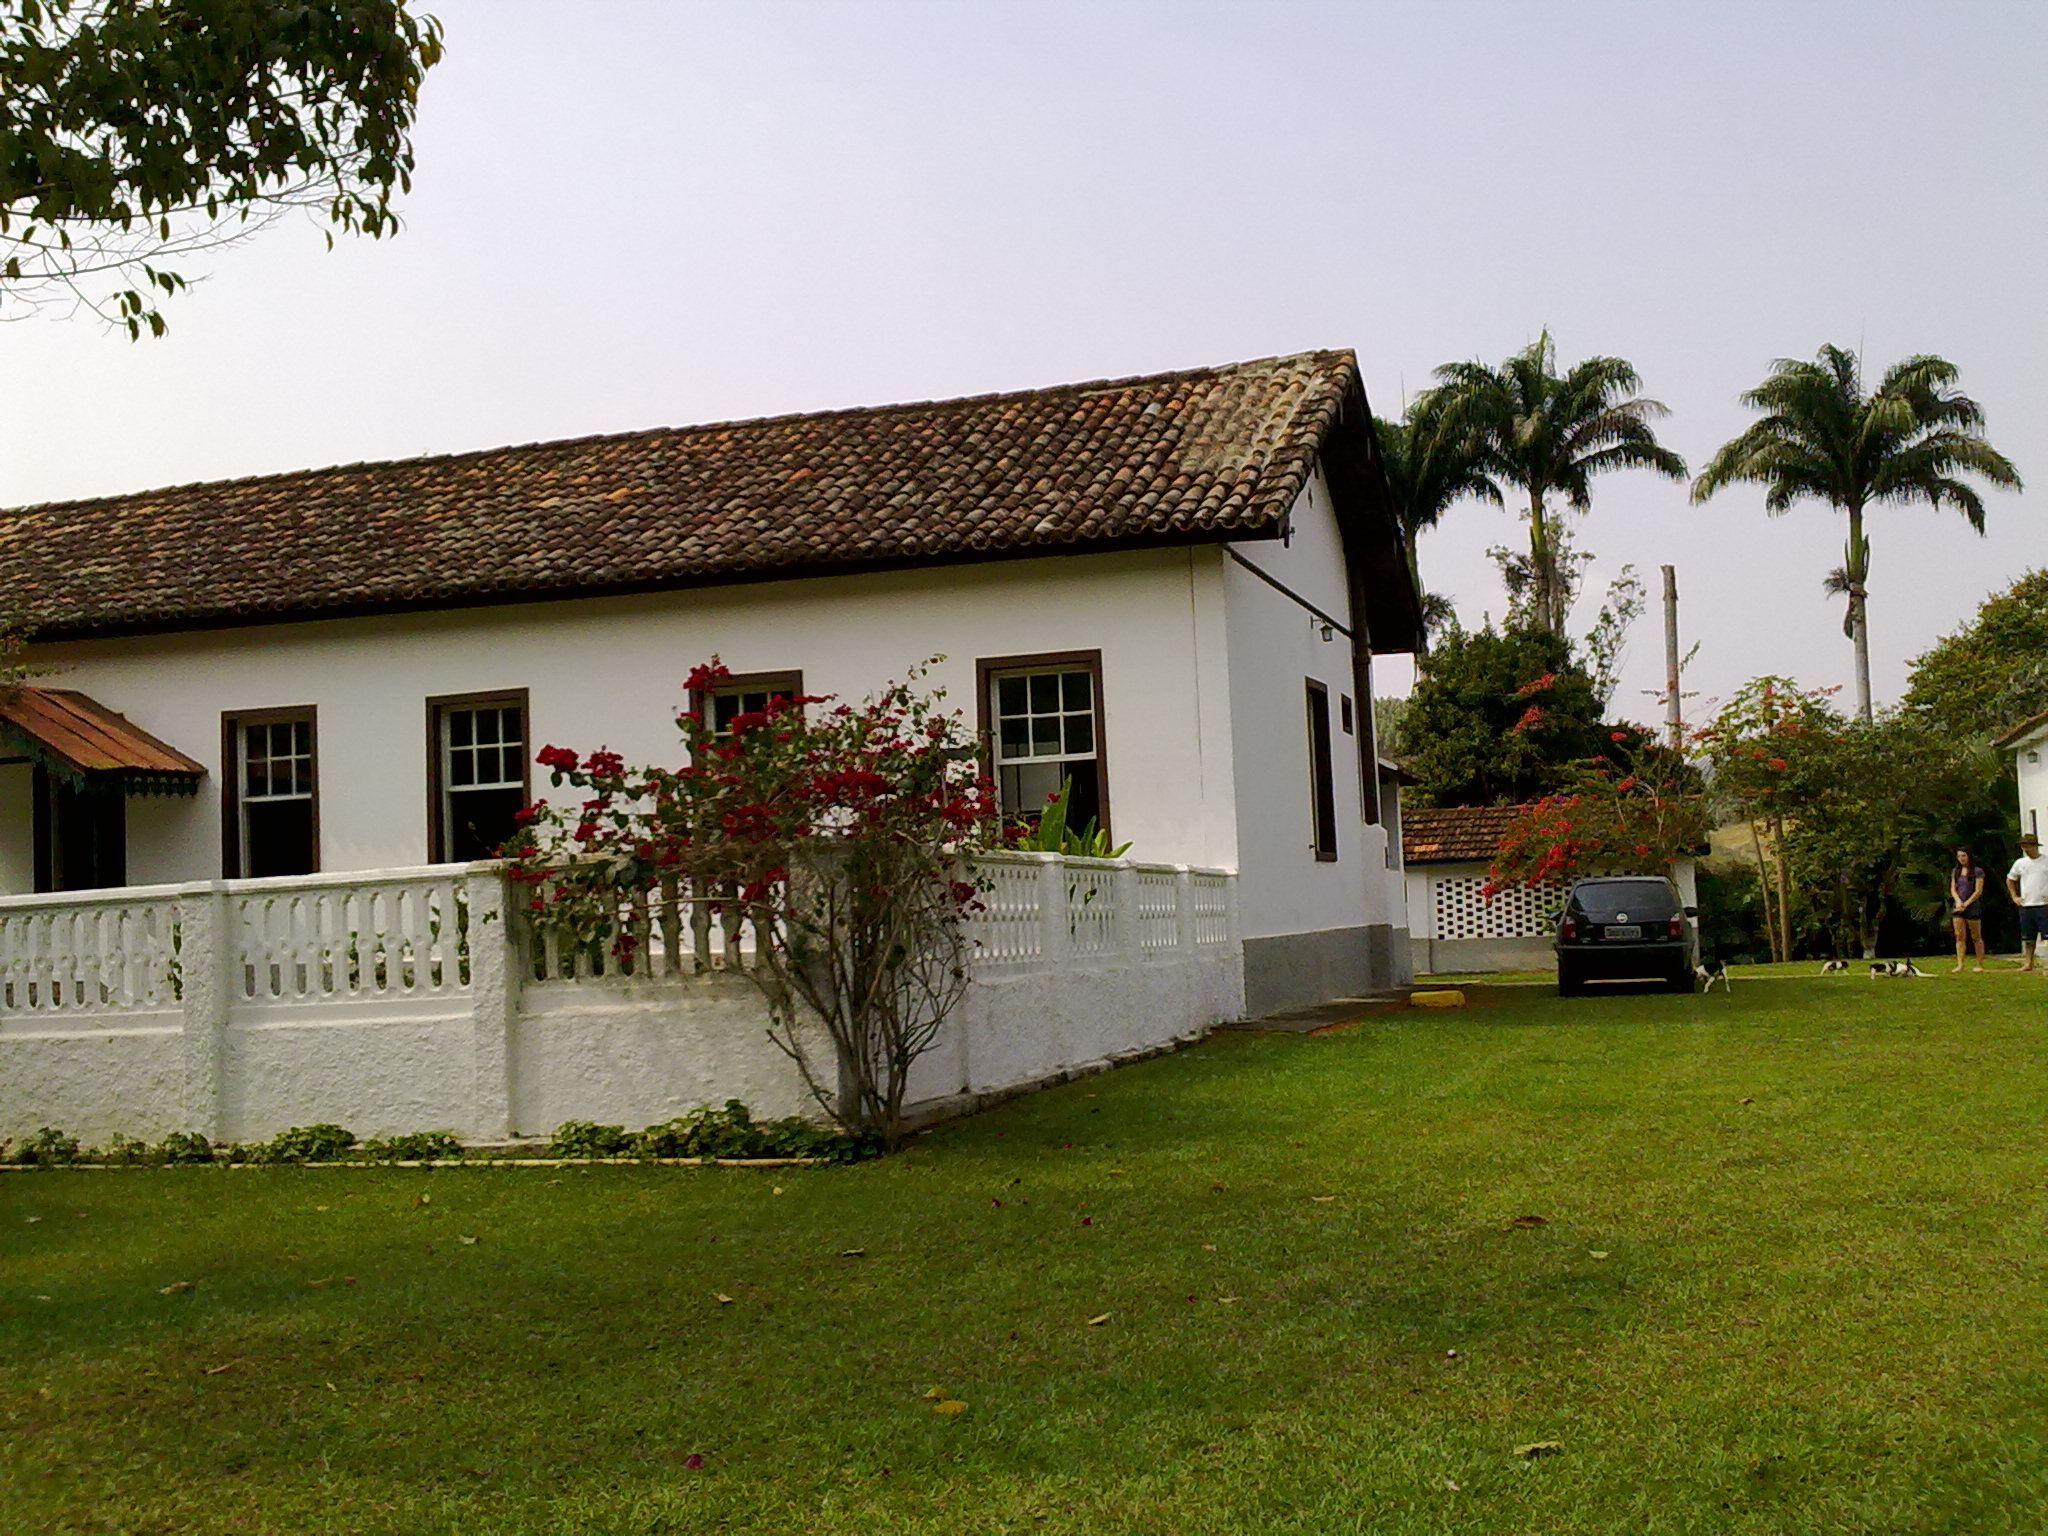
\includegraphics{./farm.jpg}
            \caption{Main house of the farm I grew up in, months before destruction.}
        \end{figure}
            --- This comes mostly from my own reflections on the meaning of home. Ever since the farm I grew up in was destroyed for the construction of a damn ca. 2010, I have felt a deeply crippling sense of homelessness.
            When in Lion Saroo states ``I'm lost,'' he states a feeling that I can deeply relate to, that of feeling ungrounded, and lacking some inherent structure that seems to be necessary for a truly human existence. This relates back to his experience of changes when returning to his hometown, which I can also relate to from going back ``home'' to find an unrecognizable patch of half-flooded land.

        \item How is the self seen in the eyes of the self? Do we only see ourselves as one of the many alter-egos that compose the other, in Lacanian terms? How do we define and see ourselves? --- This question came from my readings of Lacan's seminars, mostly for the previous essay, and from reflecting on the essay prompt.
            I feel like who we \emph{are} is always an internal, self-determining factor, \emph{i.e.} we are who we say/think we are, and from this the question of ``How does the self see itself'' follows naturally.
    \end{itemize}
    \subsection*{1 --- Essay}
    \paragraph*{Home as the incurable absence of the past}  \hspace{0pt} \\
    The Human Condition, the essential characteristics of human existence, is composed of a multitude of disparate, and often disjoin, elements. One of these elements is, inarguably, the concept of home, and the feeling of ``homeliness'' associated with it, everyone has a home, independently of whether it is physically extant or accessible. Home is fundamentally an abstract concept, it lives in our Imaginary, and it is usually define by it's absence.

    There are a plethora of concepts which can only be defined subtractively, negatively, in a relational form to it's positive counterpart; darkness is the absence of light; dryness is the absence of water; silence is the absence of sound. Home, although not entirely, behaves similarly at a conceptual level; it is much easier to know when one is not at home, than the converse. Therefore, in a sense, we define home as being the only place where we do not feel not-at-home.
As an anecdotal example, I do not feel at home in Santa Barbara, much like I did not feel at home in Lisbon, nor in Geneva, and, for the most part, not in Rio de Janeiro either; I know these places aren't home, even though I might not be sure where home is.
Here, we can connect with the timeless Talking Heads piece ``This Must Be The Place (Naive Melody)'', in which David Byrne sings ``Home is where I want to be, but I guess I'm already there.'' We see clearly here a description of this difficulty in defining and identifying home proper.

    Since we cannot, or at least so it seems, define Home directly we must do so indirectly, much like how we define darkness. At a first glance, a couple characteristics of not-home stand out. Firstly, when we are not home there is an overarching feeling of discomfort, at varying degrees. Secondly, not-home comes with a feature of unknown, of being in expectation of surprise. When one isn't home one can hope to be mistaken about locations, words, manners, etc.
David Byrne and Brian Eno touch on this issue in their 2008 joint work ``Everything That Happens Will Happen Today.'' In the opening track, titled ``Home'', Byrne sings
\begin{blocks}
Home --- where the wheels are turning\\
Home --- why I keep returning\\
Home --- where my world is breaking in two\\
Home --- with the neighbors fighting\\
Home --- always so exciting\\
Home --- were my parents telling the truth?\\
Home --- such a funny feeling\\
Home --- no-one ever speaking\\
Home --- with our bodies touching\\
Home --- and the cameras watching\\
Home --- will infect what ever you do\\
We're Home --- comes to life from outta the blue\\
\end{blocks}
Here, although hidden behind the poetical layer of the composition, we find an attempt at deciphering, and describing, the intangible that is home. Home is this multifaceted, abstract, composite ideal, and it's inherently immaterial.

In the 2016 movie Lion we see a concrete example of the immaterialness of home. When Saroo, who has been searching for his lost family and home for years, returns to his hometown he finds that everything has changed. His brother is now dead dead, his mother is old, his sister has grown, his house is now a goat stable, the language is unintelligible.
He may have found his house, and his family, but that brings he no closer to home, for the factors that form it live exclusively in the past, and therefore only exist in his memory.

In closing, Home is inevitably an entity of the past; we know what it is only when it no longer is, and therefore we can long for it. It is a painful reality of the Human Condition that we must love so fully and dearly something that we only come to truly know whence it no longer exists, it is an inalienable curse of nostalgia. Home is this incurable, unresolvable longing for that which no longer is, and which lives in ever fading states in our Imaginary.
\end{mla}
\end{document}
